% CVPR 2026 Paper Template; see https://github.com/cvpr-org/author-kit

\documentclass[10pt,twocolumn,letterpaper]{article}

%%%%%%%%% PAPER TYPE  - PLEASE UPDATE FOR FINAL VERSION
% \usepackage{cvpr}              % To produce the CAMERA-READY version
\usepackage{cvpr}      % To produce the REVIEW version
% \usepackage[pagenumbers]{cvpr} % To force page numbers, e.g. for an arXiv version

% Import additional packages in the preamble file, before hyperref
\input{preamble}
\usepackage{algorithm}
\usepackage{algpseudocode}
\usepackage{graphicx}

\setlength{\textfloatsep}{6pt}
\setlength{\floatsep}{6pt}
\setlength{\intextsep}{6pt}

% It is strongly recommended to use hyperref, especially for the review version.
% hyperref with option pagebackref eases the reviewers' job.
% Please disable hyperref *only* if you encounter grave issues, 
% e.g. with the file validation for the camera-ready version.
%
% If you comment hyperref and then uncomment it, you should delete *.aux before re-running LaTeX.
% (Or just hit 'q' on the first LaTeX run, let it finish, and you should be clear).
\definecolor{cvprblue}{rgb}{0.21,0.49,0.74}
\usepackage[pagebackref,breaklinks,colorlinks,allcolors=cvprblue]{hyperref}

%%%%%%%%% PAPER ID  - PLEASE UPDATE
\def\confYear{2026}

%%%%%%%%% TITLE - PLEASE UPDATE
\title{Exploring Hallucination-Aware Extensions of HIRE for LVLMs}

%%%%%%%%% AUTHORS - PLEASE UPDATE
\author{Seongrae Noh\\
---------\\
{\tt\small -----------@gmail.com}
\and
Hyowone Woo\\
-----------------\\
{\tt\small ---------------@gmail.com}
\and
Sangheum Jo\\
2026020945\\
{\tt\small sanghuem20@gmail.com}
% For a paper whose authors are all at the same institution,
% omit the following lines up until the closing ``}''.
% Additional authors and addresses can be added with ``\and'',
% just like the second author.
% To save space, use either the email address or home page, not both
}

\begin{document}
\maketitle
\begin{abstract}
Base on hire, we try vti and interpretablilty
\end{abstract}   

\section{Introduction}
Multimodal Large Language Models (LVLMs) have achieved remarkable progress in image understanding by leveraging the world knowledge of Large Language Models (LLMs). As a result, LVLMs can be applied to a wider range of vision-language tasks with stronger reasoning capabilities.

However, LVLMs still suffer from hallucinations, generating responses that describe non-existent objects or incorrectly interpret visual content. Such hallucinations reduce model reliability, motivating extensive research on hallucination mitigation.

Recent studies assume that hallucination-related information can be distinguished in hidden representation spaces and have achieved promising results through contrastive learning and representation editing. However, these approaches typically require additional training and often construct hallucination data based on the observation that hallucinations occur more frequently under degraded image quality.

In this project, we adopt a training-free hallucination mitigation framework and further introduce an additional analysis module to investigate hallucination-related representations. 


\section{Related Work}

\subsection{HIRE}

Recent studies have shown that hallucination-related information can be identified in the hidden representations of LVLMs. Based on this observation, HIRE \citep{suo2026hallucination} proposes a representation-level hallucination manipulation framework consisting of an editor and a router.

HIRE learns to disentangle semantic and hallucination-related representations through image perturbation. Clean and perturbed images are encoded into latent representations, and a clustering objective is used to separate hallucination-related and reliable latent representations while preserving semantic information. Based on the learned representation space, HIRE derives editing directions that can either suppress or amplify hallucination behavior through a controllable editing scale.

To improve efficiency, HIRE further introduces a router that selectively applies editing to a subset of tokens. The router is trained using Dynamic Preference Optimization with randomly generated editing trajectories, enabling efficient hallucination mitigation while reducing computational cost.

Although HIRE achieves strong hallucination mitigation performance, it requires additional training for representation editing and routing. Furthermore, the relationship between perturbation-induced representations and hallucination formation remains insufficiently explained.



\subsection{VTI}
model training free but week sementic retain so projection

\subsection{Interpretable Model Structure}

Interpretable neural network architectures have been widely studied to improve model transparency. One representative approach is the Concept Bottleneck Model (CBM) \citep{koh2020concept}, which introduces an intermediate concept layer between hidden representations and final predictions. By explicitly modeling concept activations, CBMs enable interpretation of how information contributes to model decisions.

However, CBMs require concept-level supervision, which is unavailable for hallucination-related representations in LVLM hidden spaces. To address this limitation, we adopt prototype learning methods \citep{singh2021these, kim2022vit}. Prototype learning constructs representative prototypes for each class and learns discriminative feature patterns directly from hidden representations. As a result, meaningful concepts can be extracted without explicit representation-level annotations.

In this work, we use prototype learning to construct representation-level hallucination concepts and train a CBM on the resulting prototype activations. This enables concept-level analysis of hallucination-related representations.




\section{Method}
Here we talk about what we do.

----------------------------------------------------------
\subsection{Sementic Representation in Training free}

We try extend two way, traintig free hallusioanation. Make new tex at sec folder and input here

\subsubsection{Problem Setup}

use vti

\subsubsection{Prompt Filtering via Subspace Projection}

wkwjeifjakljdlkfa

--------------------------------------------------------------------
\subsection{Representation-level Hallucination Interpretability}

Existing hallucination mitigation methods focus on reducing hallucinated outputs but provide limited interpretability of hallucination-related representations. To address this limitation, we introduce a prototype-based CBM that learns hallucination concepts in hidden representation space and analyzes representations through concept activations.


\subsubsection{Prototype-based Concept Learning}

CBMs require concept-level supervision, but hallucination concepts are not explicitly annotated in hidden representation space. To obtain interpretable concepts, we learn layer-wise prototypes corresponding to Safe and Existence hallucination categories and construct a prototype bank across all transformer layers.

Given a hidden representation $h_i^l$ from transformer layer $l$, a prototype encoder projects it into a lower-dimensional embedding space $z_i^l$. The encoded representation is compared with learnable concept prototypes using cosine similarity $s_{i,l,c}$, where $c \in \{\text{safe}, \text{existence}\}$ denotes the concept category.

To obtain discriminative concept representations, we jointly optimize classification, clustering, and separation objectives. The classification loss encourages correct concept assignment, the cluster loss pulls samples toward the corresponding prototype, and the separation loss pushes samples away from other concept prototypes.

Algorithm~\ref{alg:layerwise_prototype_learning} summarizes the prototype learning procedure.

\begin{algorithm}[!t]
\caption{Layer-wise Prototype Learning for Safe / Existence Concepts}
\label{alg:layerwise_prototype_learning}
\begin{algorithmic}[1]
\Require Layer-wise hidden representations $\mathcal{H}=\{(H_i, y_i)\}_{i=1}^{N}$, where $y_i \in \{\text{safe}, \text{existence}\}$
\Require $H_i = [h_i^{1}, h_i^{2}, \dots, h_i^{L}]$, where $h_i^{l}\in\mathbb{R}^{d_h}$
\Require Learnable layer-wise prototypes $\{p_{l,c}\}_{l=1,c\in\{\text{safe},\text{exist}\}}^{L}$
\Require Prototype encoder $f_\theta:\mathbb{R}^{d_h}\rightarrow\mathbb{R}^{d_z}$

\For{each training epoch}
    \For{each mini-batch $\mathcal{B}\subset\mathcal{H}$}
        \For{each sample $(H_i,y_i)\in\mathcal{B}$}
            \For{each layer $l=1,\dots,L$}
                \State Encode layer representation
                \[
                    z_i^l \leftarrow f_\theta(h_i^l)
                \]

                \State Normalize representation and prototypes
                \[
                    \tilde{z}_i^l \leftarrow \frac{z_i^l}{\|z_i^l\|_2},
                    \quad
                    \tilde{p}_{l,c} \leftarrow \frac{p_{l,c}}{\|p_{l,c}\|_2}
                \]

                \State Compute prototype similarity
                \[
                    s_{i,l,c}
                    =
                    (\tilde{z}_i^l)^\top \tilde{p}_{l,c}
                \]
            \EndFor

            \State Aggregate layer-wise similarities
            \[
                \ell_{i,c}
                =
                \frac{1}{L}
                \sum_{l=1}^{L}
                s_{i,l,c}
            \]

            \State Compute prototype loss
            \[
                \mathcal{L}_{i}
                =
                \mathcal{L}_{cls}^{i}
                +
                \lambda_c \mathcal{L}_{cluster}^{i}
                +
                \lambda_s \mathcal{L}_{sep}^{i}
            \]
        \EndFor

        \State Compute mini-batch loss
        \[
            \mathcal{L}_{proto}
            =
            \frac{1}{|\mathcal{B}|}
            \sum_{(H_i,y_i)\in\mathcal{B}}
            \mathcal{L}_i
        \]

        \State Update encoder and prototypes
    \EndFor
\EndFor

\State \Return $f_\theta,\{p_{l,c}\}$
\end{algorithmic}
\end{algorithm}

\subsubsection{Concept Bottleneck Module}

After learning concept prototypes, we train a CBM. Instead of directly predicting hallucination labels from hidden representations, the CBM estimates concept activations from prototype similarities, providing an interpretable bottleneck between representations and hallucination prediction.

For each sample, prototype similarities from all transformer layers are aggregated into a concept vector $v_i$. The vector is processed by an MLP $g_\phi$, and concept activations $\hat{c}_i$ are obtained through a sigmoid function.

To improve concept interpretability, we optimize the CBM using both prediction and concept supervision objectives. Binary cross-entropy encourages correct concept prediction, while sparsity regularization discourages multiple concepts from being activated simultaneously.

\[
\mathcal{L}_{CBM}
=
\mathcal{L}_{CE}
+
\lambda_{BCE}\mathcal{L}_{BCE}
+
\lambda_{sparse}\mathcal{L}_{sparse}
\]

Algorithm~\ref{alg:layerwise_cbm_training} summarizes the CBM training procedure. The learned concept activations provide an interpretable view of hidden representations and enable hallucination analysis at the representation level. By preserving layer-wise prototype similarities, the proposed framework allows investigation of how hallucination-related information evolves.

\begin{algorithm}[!t]
\caption{Layer-wise Concept Bottleneck Training with Prototype Activations}
\label{alg:layerwise_cbm_training}
\begin{algorithmic}[1]
\Require Layer-wise hidden representations $\mathcal{H}$
\Require Trained prototype bank $\{p_{l,c}\}$
\Require Prototype encoder $f_\theta$
\Require Concept bottleneck layer $g_\phi$

\For{each training epoch}
    \For{each mini-batch}
        \For{each sample}
            \For{each layer $l$}
                \State Encode representation
                \[
                z_i^l=f_\theta(h_i^l)
                \]

                \State Compute similarity
                \[
                s_{i,l,c}
                =
                \cos(z_i^l,p_{l,c})
                \]
            \EndFor

            \State Aggregate concept vector
            \[
            v_i
            =
            \left[
            \frac{1}{L}\sum_l s_{i,l,1},
            \dots,
            \frac{1}{L}\sum_l s_{i,l,K}
            \right]
            \]

            \State Predict concept activations
            \[
            \hat{c}_i
            =
            \sigma(g_\phi(v_i))
            \]

            \State Compute CBM loss
        \EndFor

        \State Update CBM parameters
    \EndFor
\EndFor

\State \Return $g_\phi$
\end{algorithmic}
\end{algorithm}



\section{Experiments}

We test our project

\subsection{Hallucination Interpretability}

\subsubsection{Experimental Setup}

We evaluate the CBM on the generative subset of the AMBER dataset using LLaVA-1.5-7B and HIRE.

The dataset\citep{wang2023amber} contains 9,848 Existence hallucination samples and 5,599 Safe samples. Hidden representations are extracted from all 32 transformer layers, and prototype similarity is measured using cosine similarity.



\subsubsection{CBM Validation}

\paragraph{Minimal Impact on Generation}
Table~\ref{tab:chair_results} reports CHAIR and Recall scores on the COCO validation subset. 
As expected, introducing the CBM module causes negligible changes in generation performance. The differences between the original models and their CBM counterparts remain minimal across all metrics. This is expected because the proposed framework is designed for representation analysis rather than hallucination mitigation.

\begin{table}[t]
\centering
\caption{Hallucination evaluation on the COCO validation subset (100 images). Lower CHAIRs/CHAIRi is better, while higher Recall is better.}
\begin{tabular}{lccc}
\hline
Model & CHAIRs $\downarrow$ & CHAIRi $\downarrow$ & Recall $\uparrow$ \\
\hline
LLaVA      & 0.5200 & 0.1409 & 0.7940 \\
HIRE       & 0.5000 & 0.1275 & 0.7209 \\
LLaVA+CBM  & 0.5200 & 0.1417 & 0.7859 \\
HIRE+CBM   & 0.5000 & 0.1276 & 0.7127 \\
\hline
\end{tabular}
\label{tab:chair_results}
\end{table}


\paragraph{Correlation with Hallucination Metrics}
To investigate whether the learned concepts are related to hallucination behavior, we compute correlations between CBM concept activations, prototype similarities, and CHAIR metrics. 
Table~\ref{tab:cbm_chair_corr} presents the correlation coefficients. Although the correlations are moderate, all metrics exhibit positive relationships with both CHAIRi and CHAIRs. These observations suggest that the learned concepts capture hallucination-related characteristics in representation space.

\begin{table}[t]
\centering
\caption{Correlation between CBM Existence Metrics and CHAIR Scores}
\label{tab:cbm_chair_corr}
\begin{tabular}{lcc}
\hline
\textbf{Metric} & \textbf{CHAIRi} & \textbf{CHAIRs} \\
\hline
Avg. Existence Score      & 0.274 & 0.279 \\
Max. Existence Score      & 0.291 & 0.330 \\
Avg. Prototype Similarity & 0.273 & 0.280 \\
Max. Prototype Similarity & 0.290 & 0.319 \\
\hline
\end{tabular}
\end{table}



\subsubsection{Representation Analysis}

\paragraph{Consistent Concept Separation}

To investigate whether the learned concepts are consistently separated, we analyze prototype margins and cross-layer prototype similarities.

\begin{figure}[t]
\centering
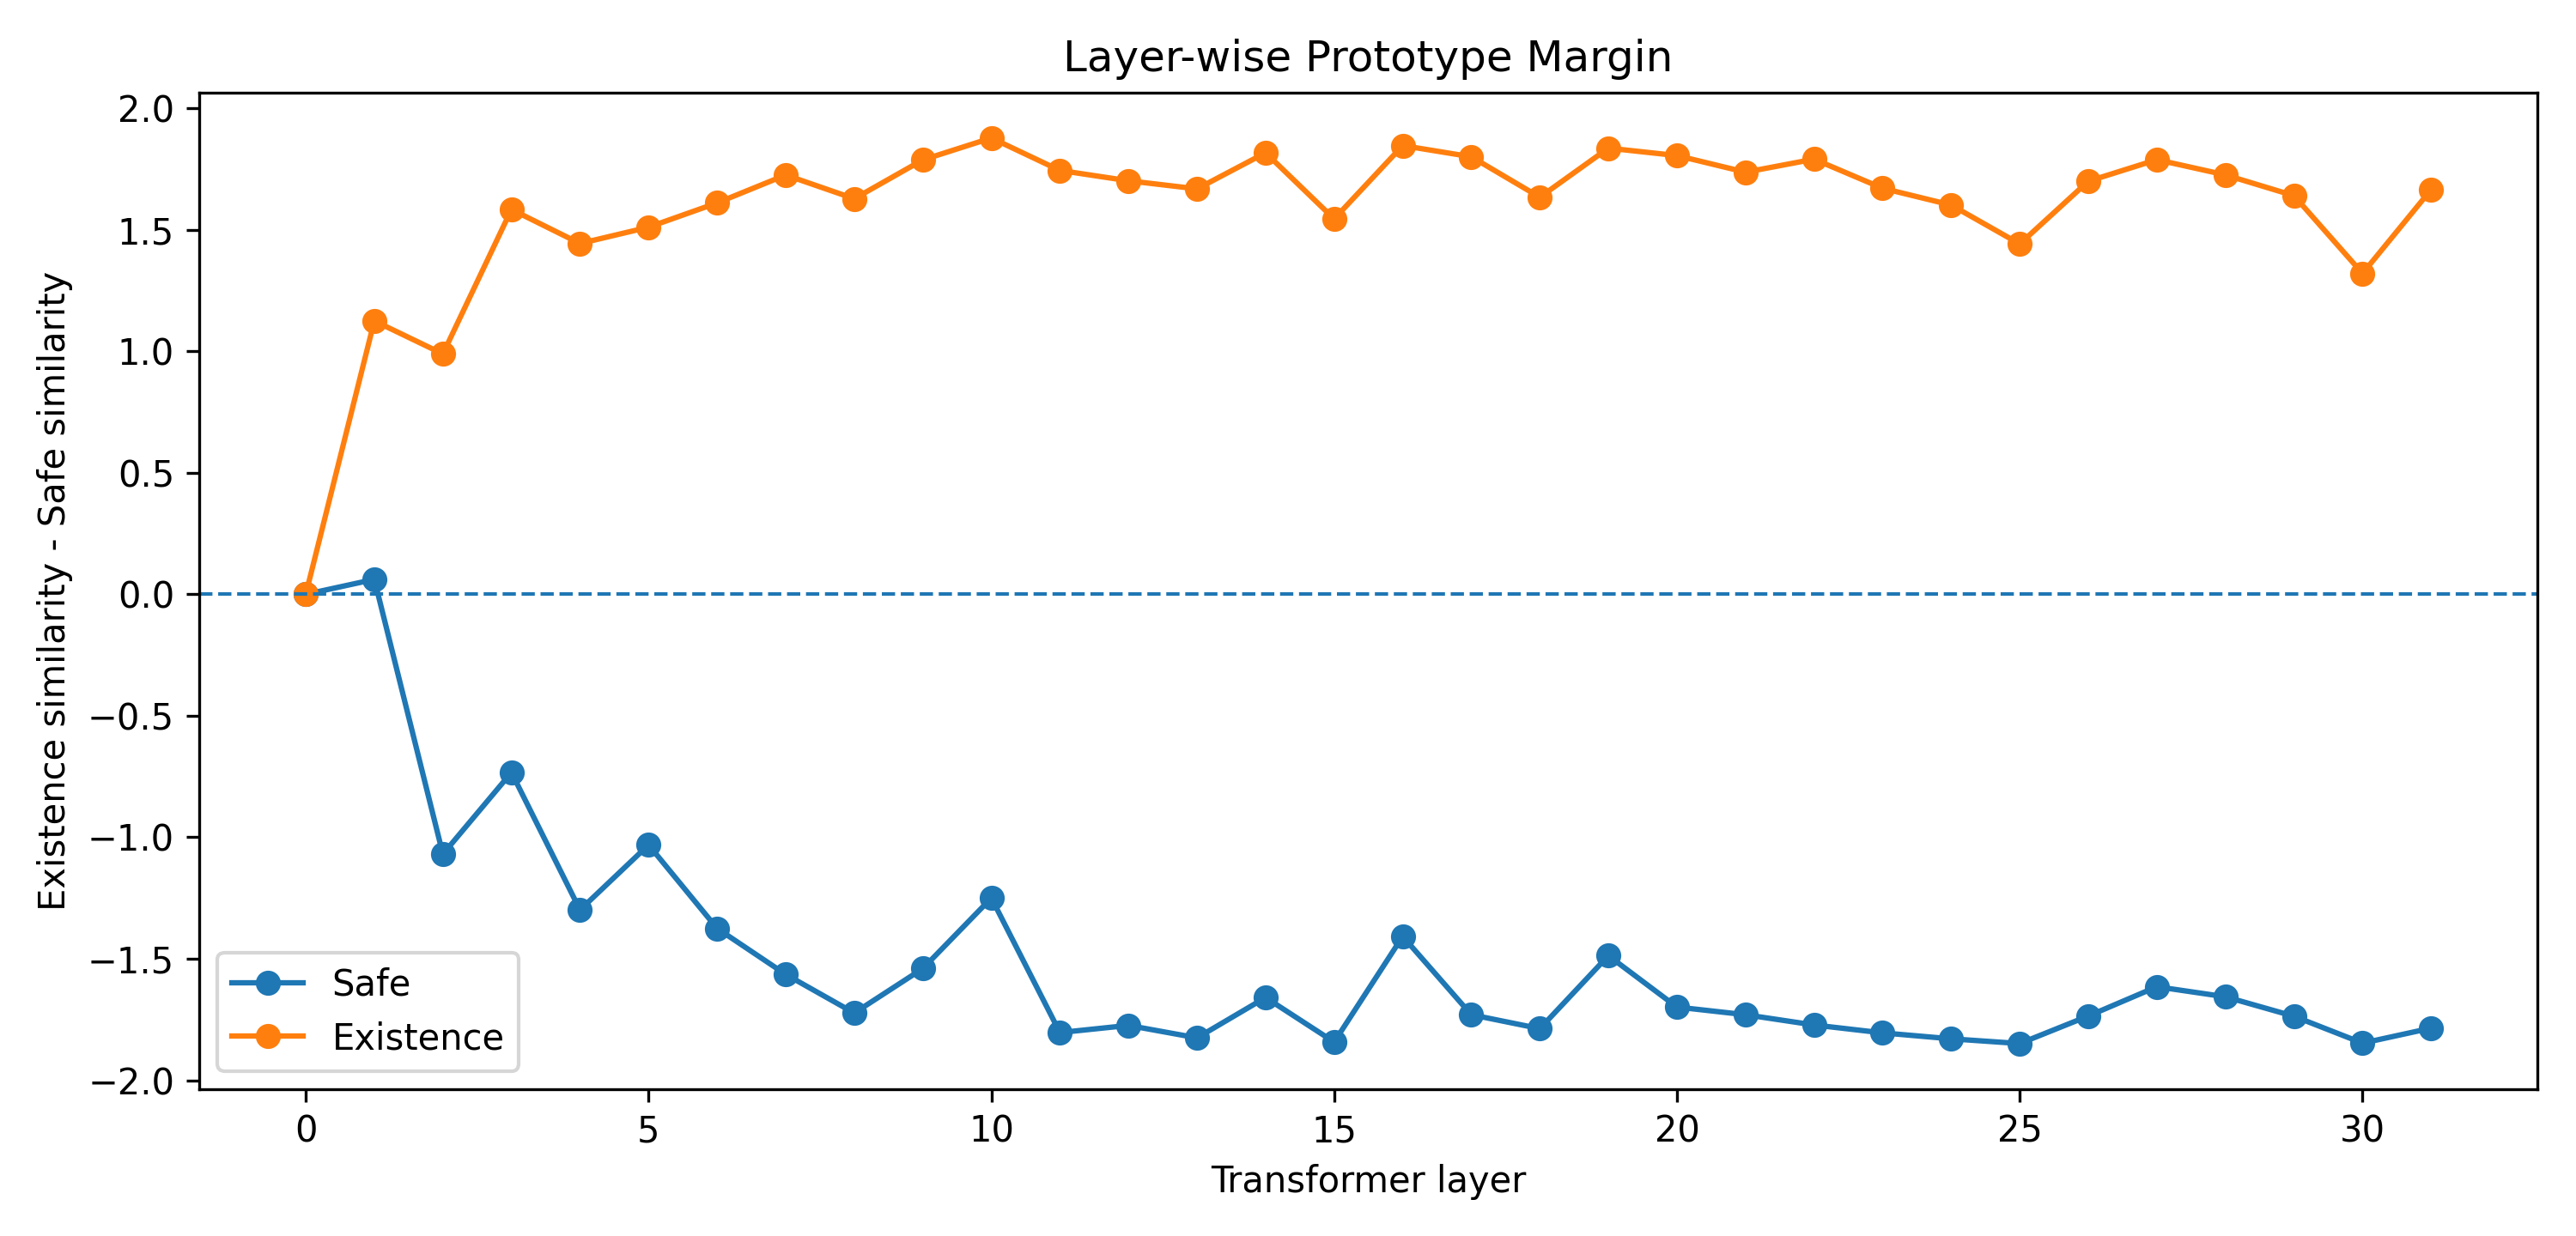
\includegraphics[width=0.48\linewidth]{figures/layerwise_margin.png}
\hfill
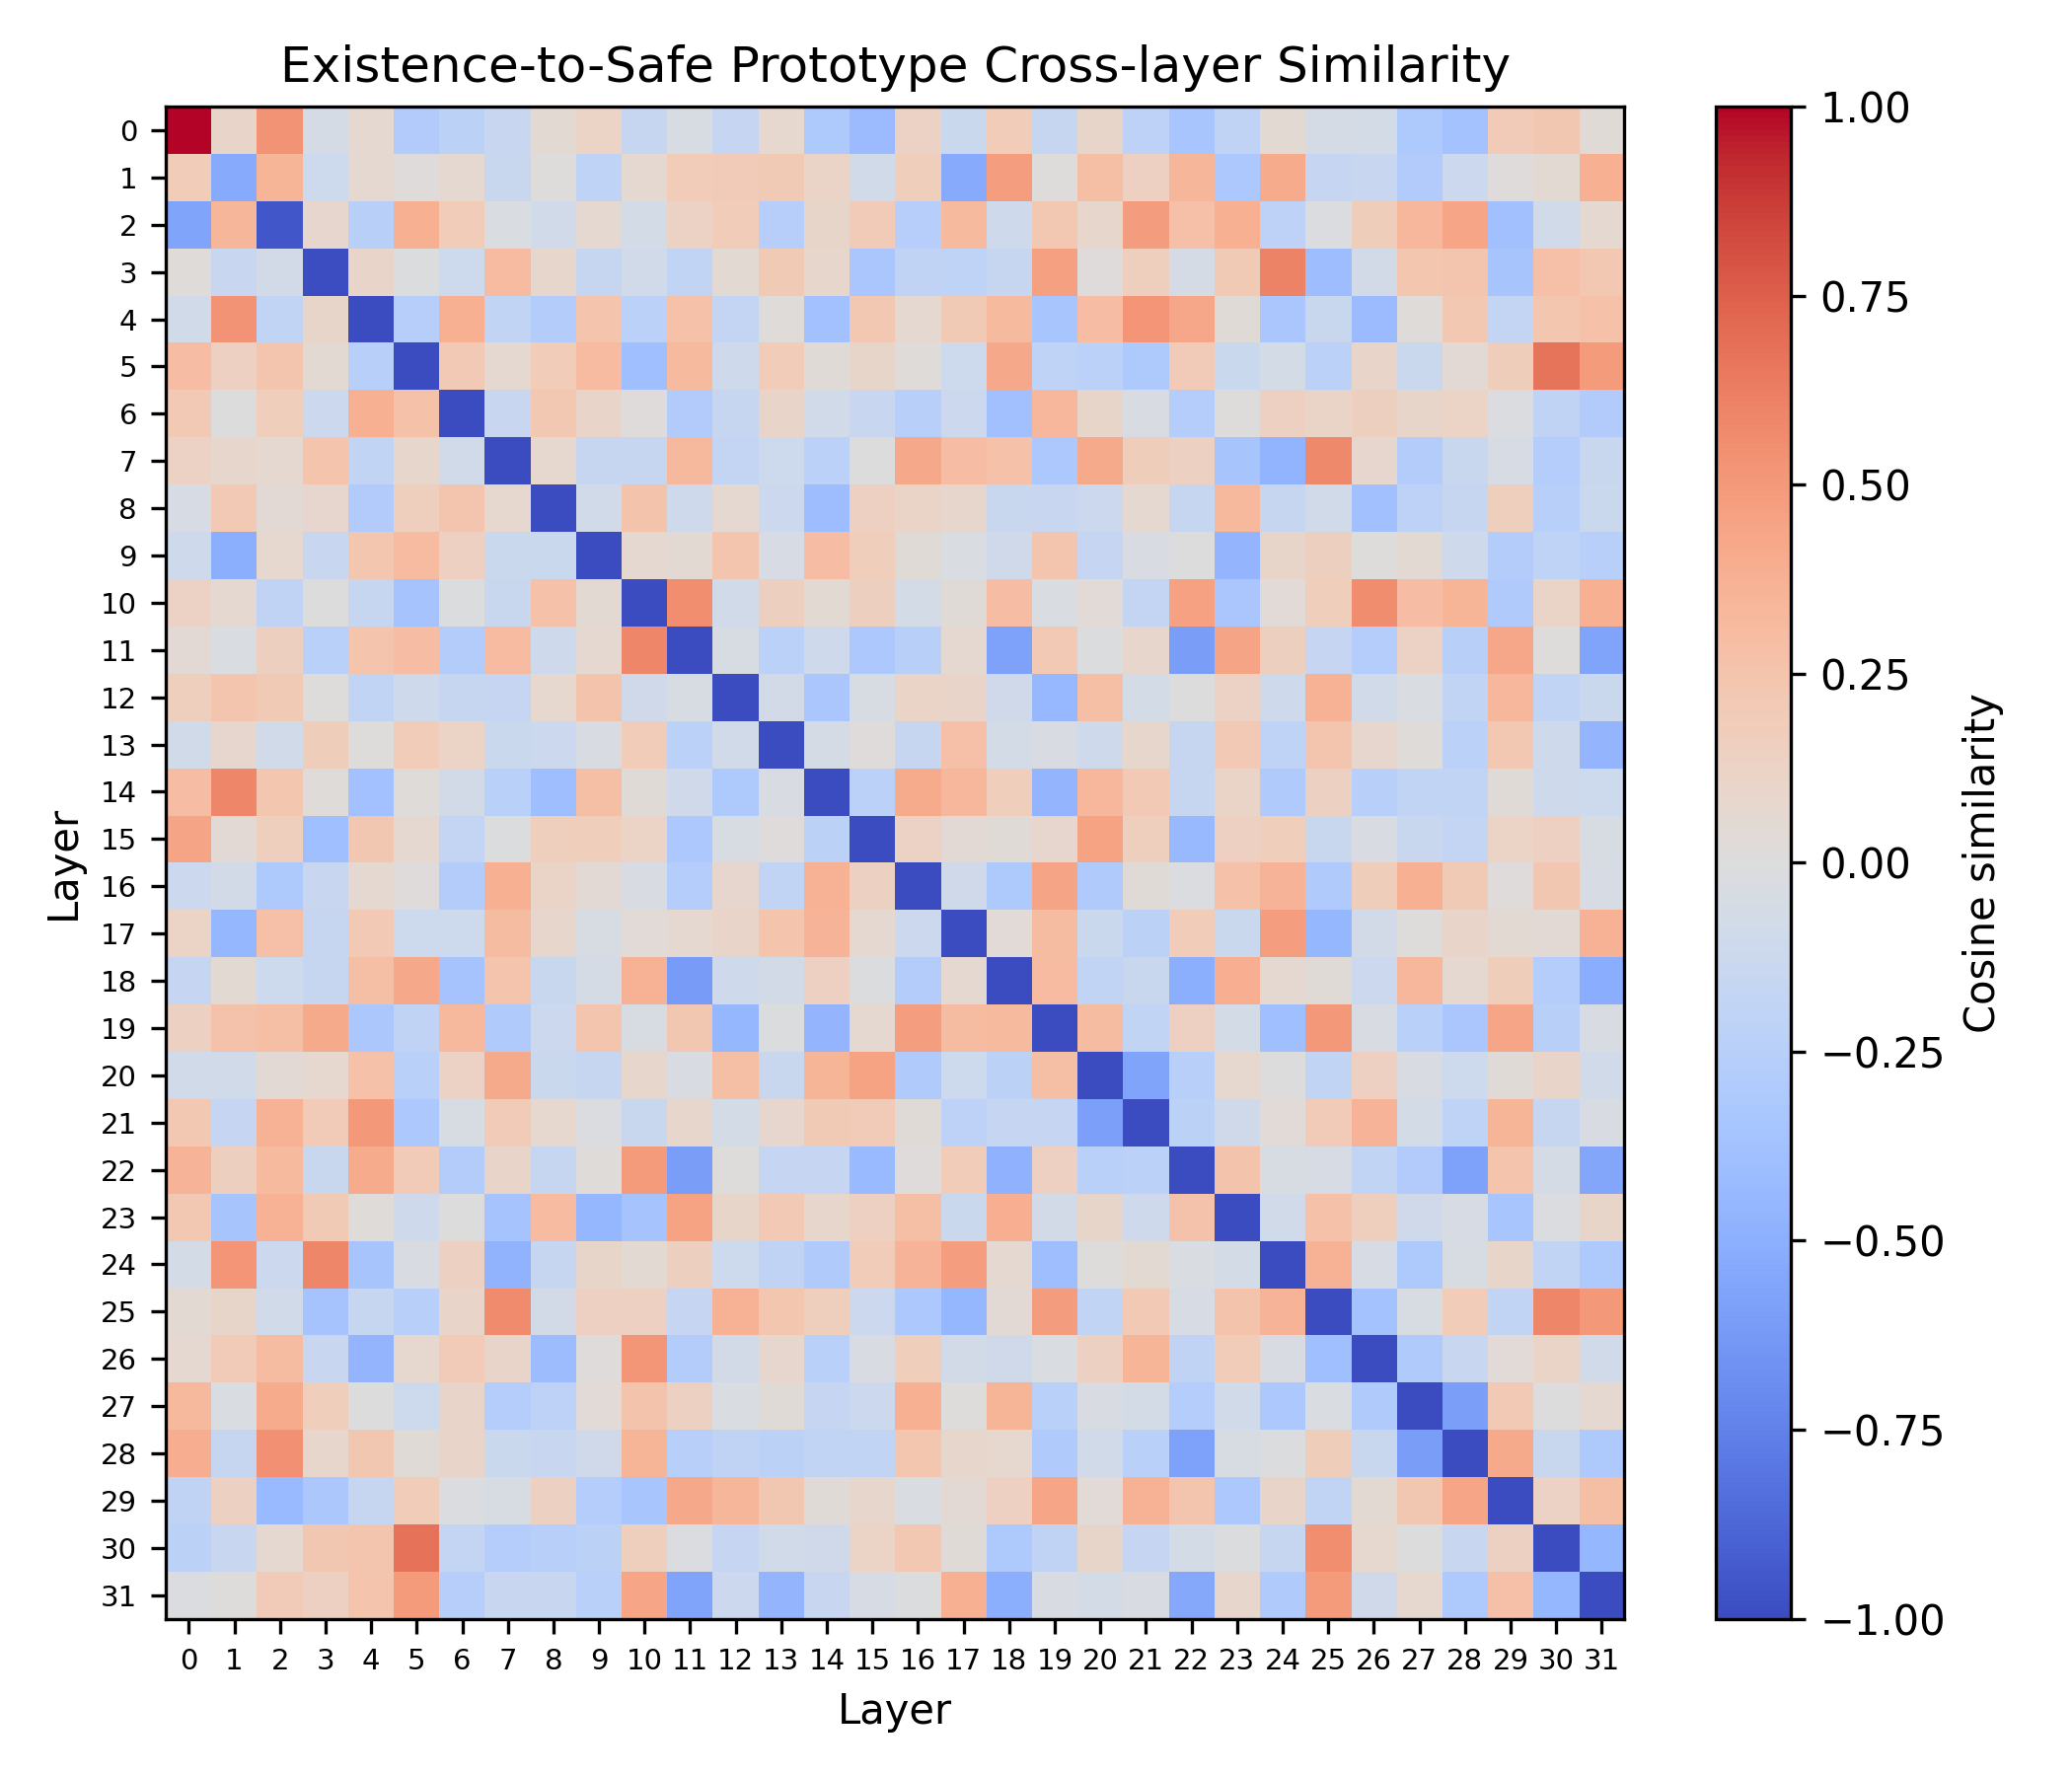
\includegraphics[width=0.48\linewidth]{figures/cross_layer_similarity.png}
\caption{Concept separation analysis. Left: layer-wise prototype margin between Safe and Existence concepts. Right: cross-layer prototype similarity matrix.}
\label{fig:concept_separation}
\end{figure}

As shown in Figure~\ref{fig:concept_separation}, Safe and Existence concepts begin to separate after approximately the third transformer layer, and the margin converges around the eighth layer. This indicates that the learned prototypes capture distinct representation patterns associated with hallucination behavior.

The cross-layer similarity matrix further shows strong diagonal patterns, suggesting that each layer learns a stable and distinct concept representation. Together, these results indicate consistent concept separation throughout the network.

\paragraph{Stronger Signals in Deeper Layers}

We further analyze prototype activation distributions across early, middle, and late transformer layers.

\begin{figure}[t]
\centering
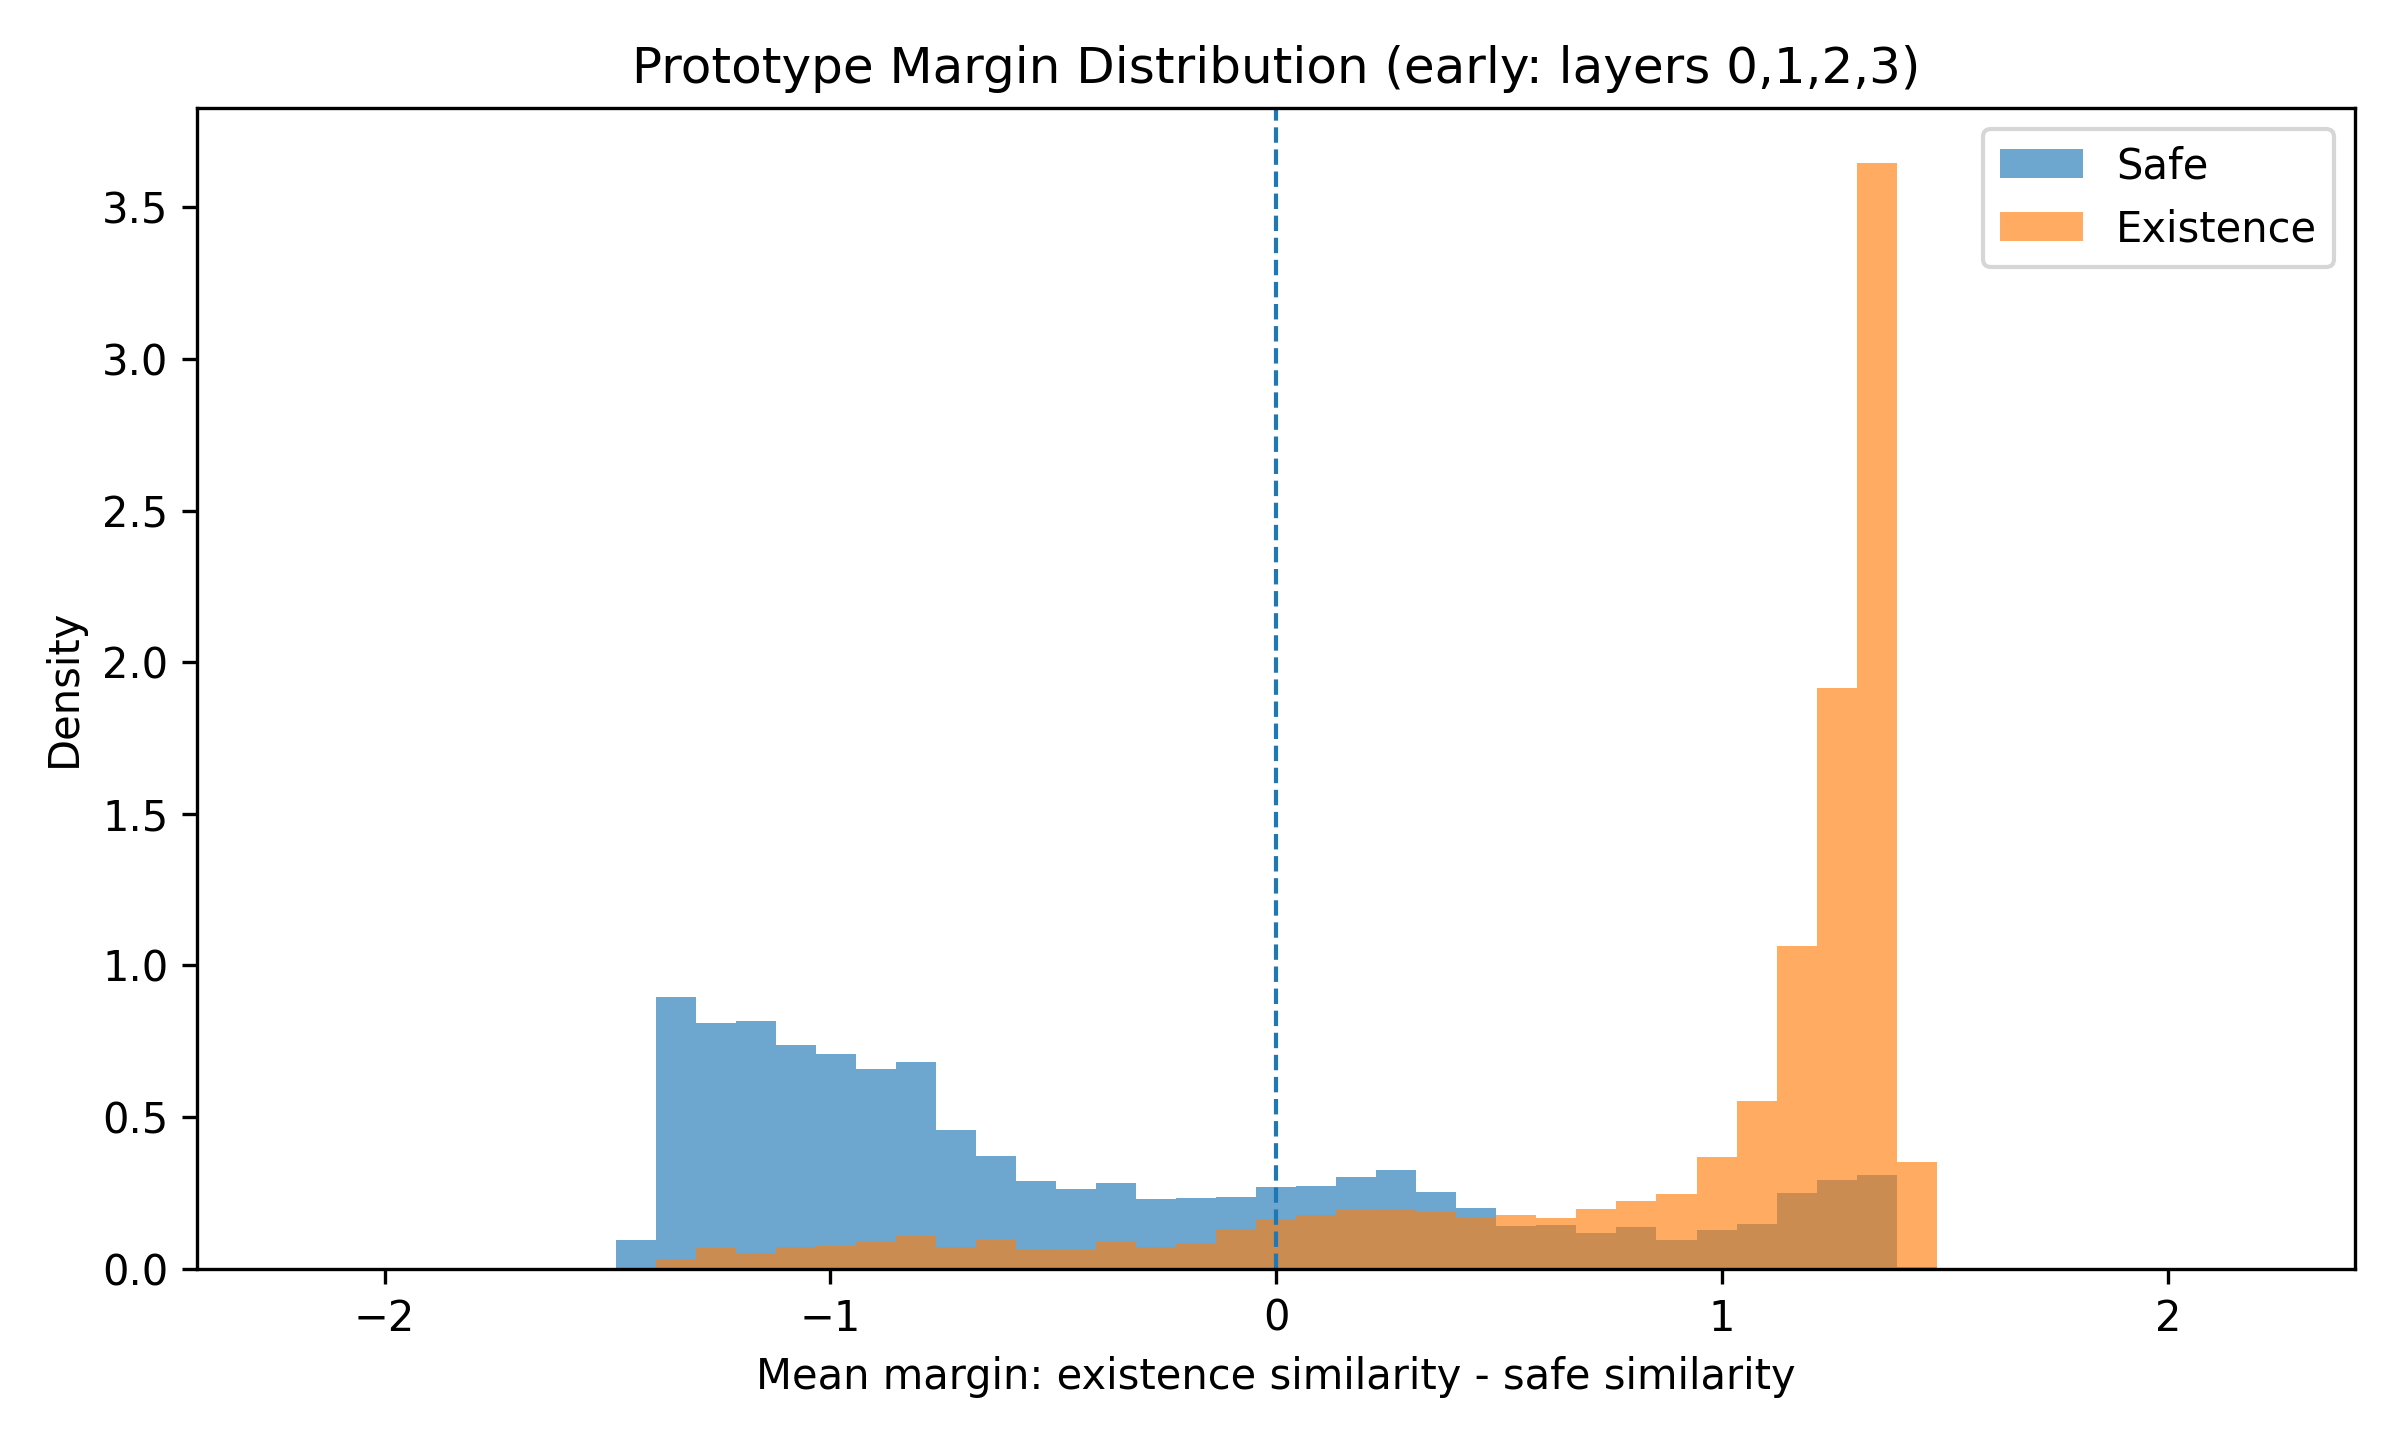
\includegraphics[width=0.32\linewidth]{figures/distribution_early.png}
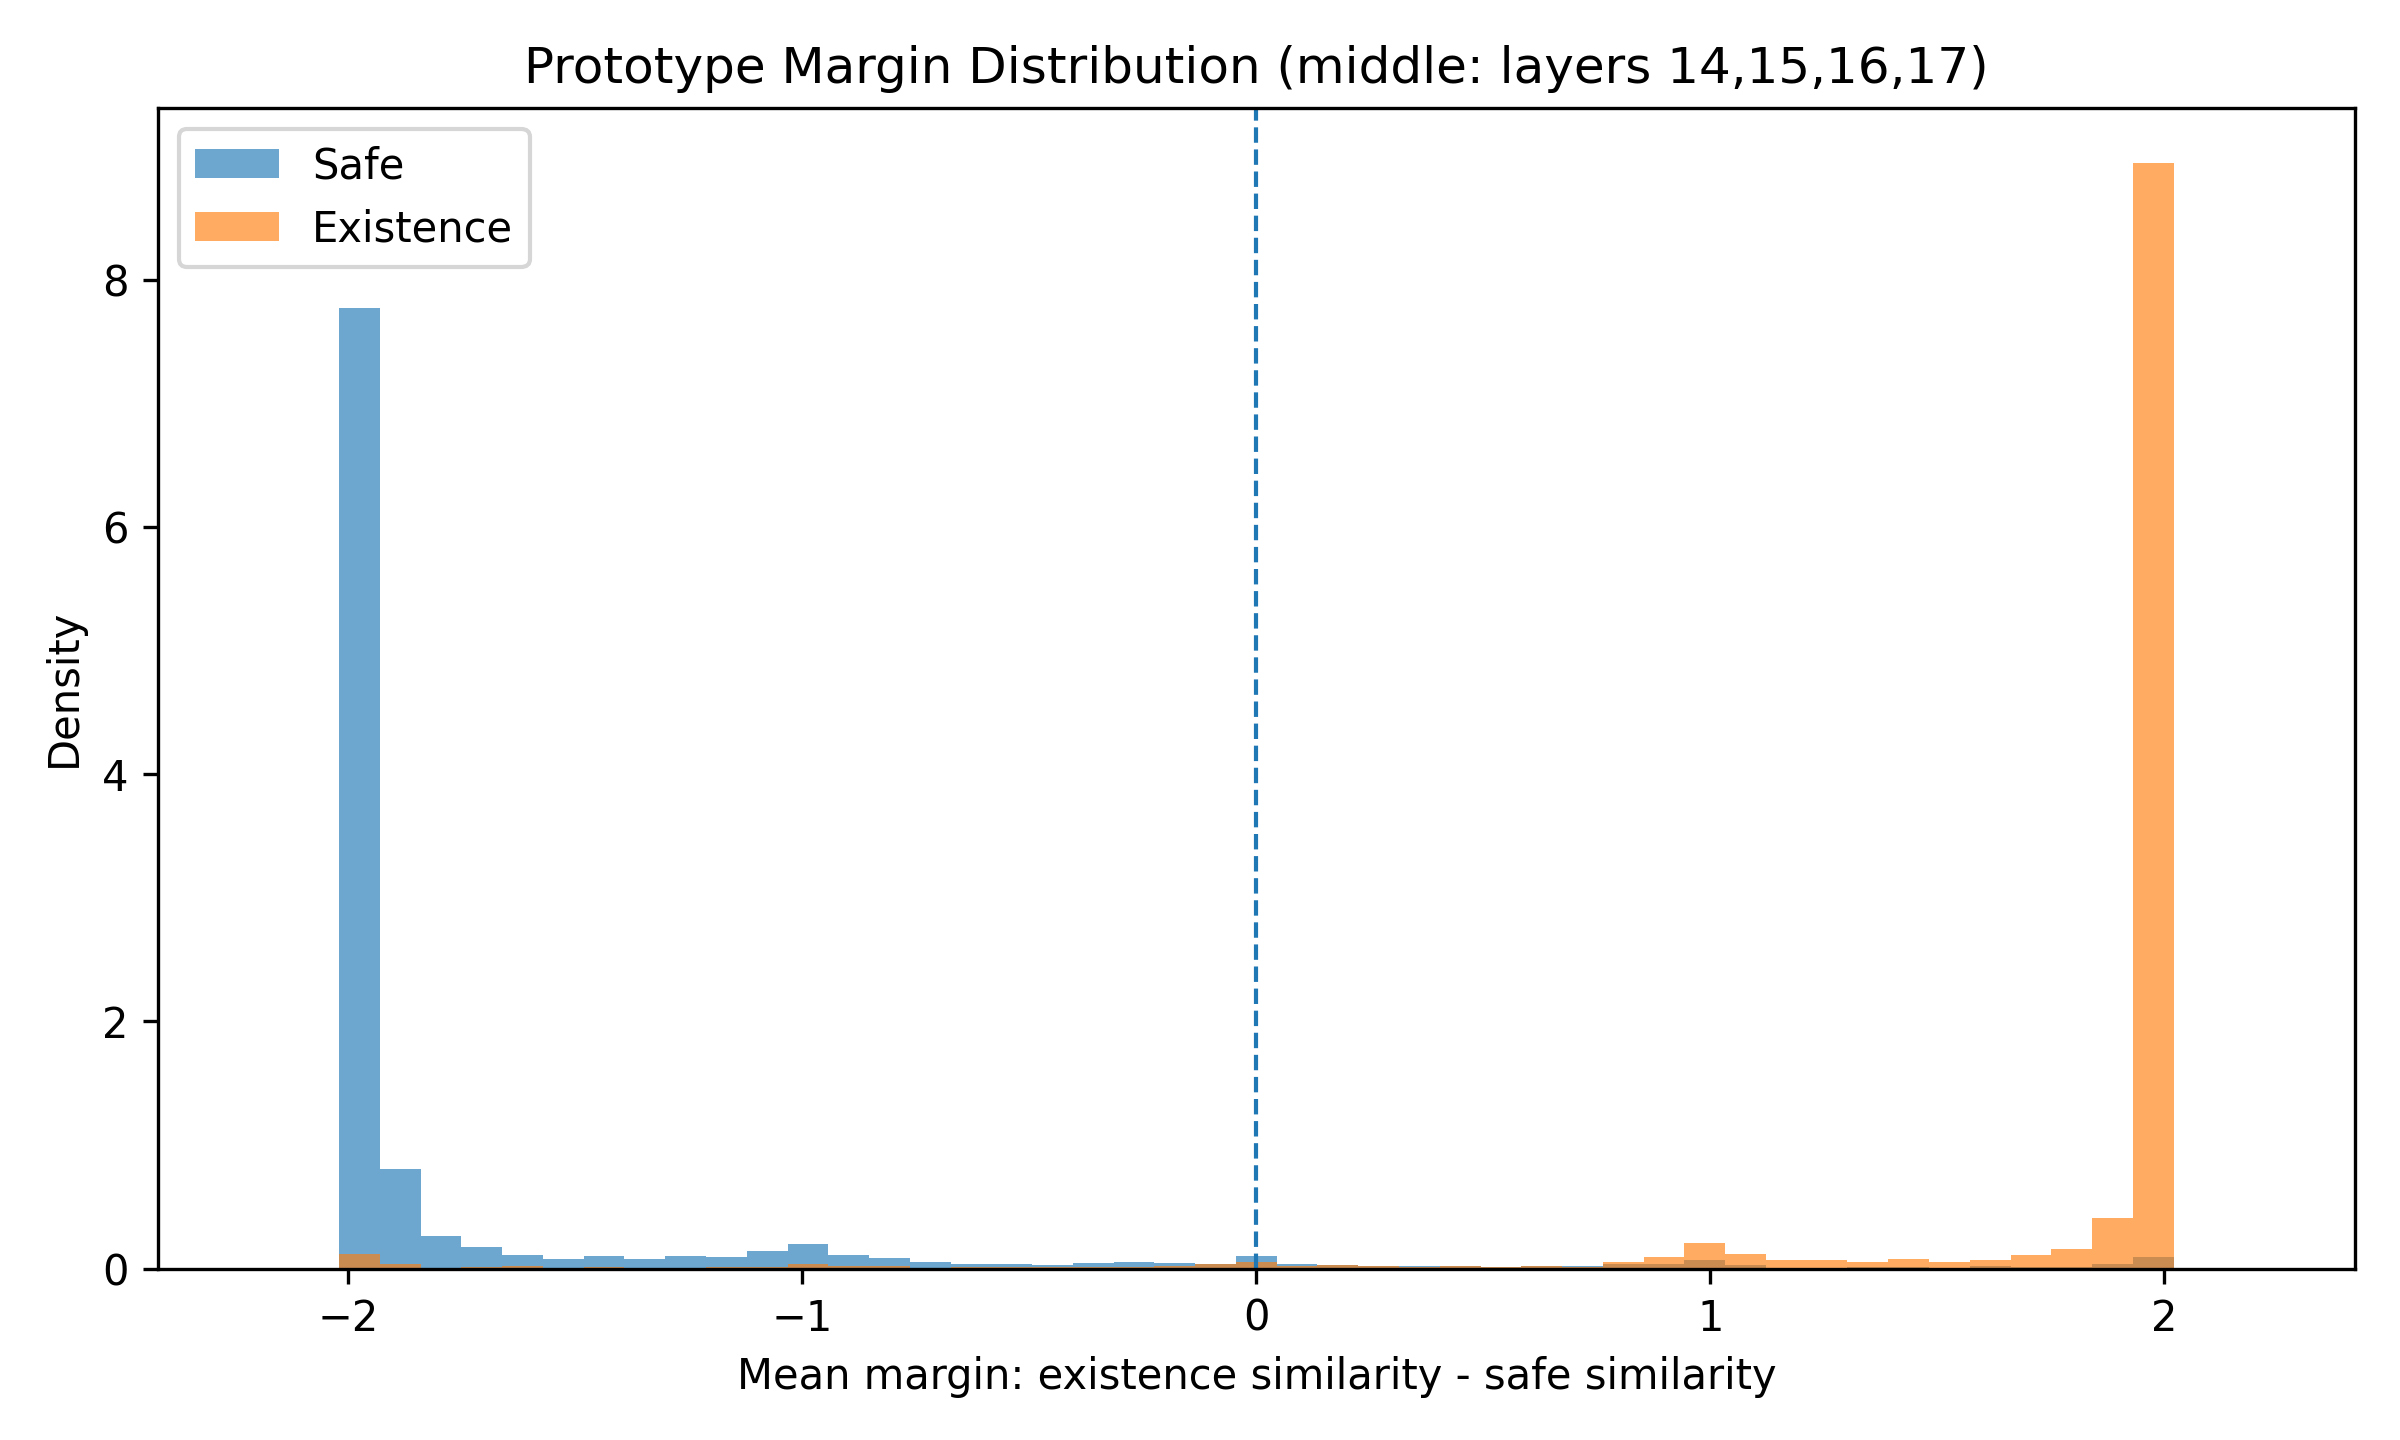
\includegraphics[width=0.32\linewidth]{figures/distribution_middle.png}
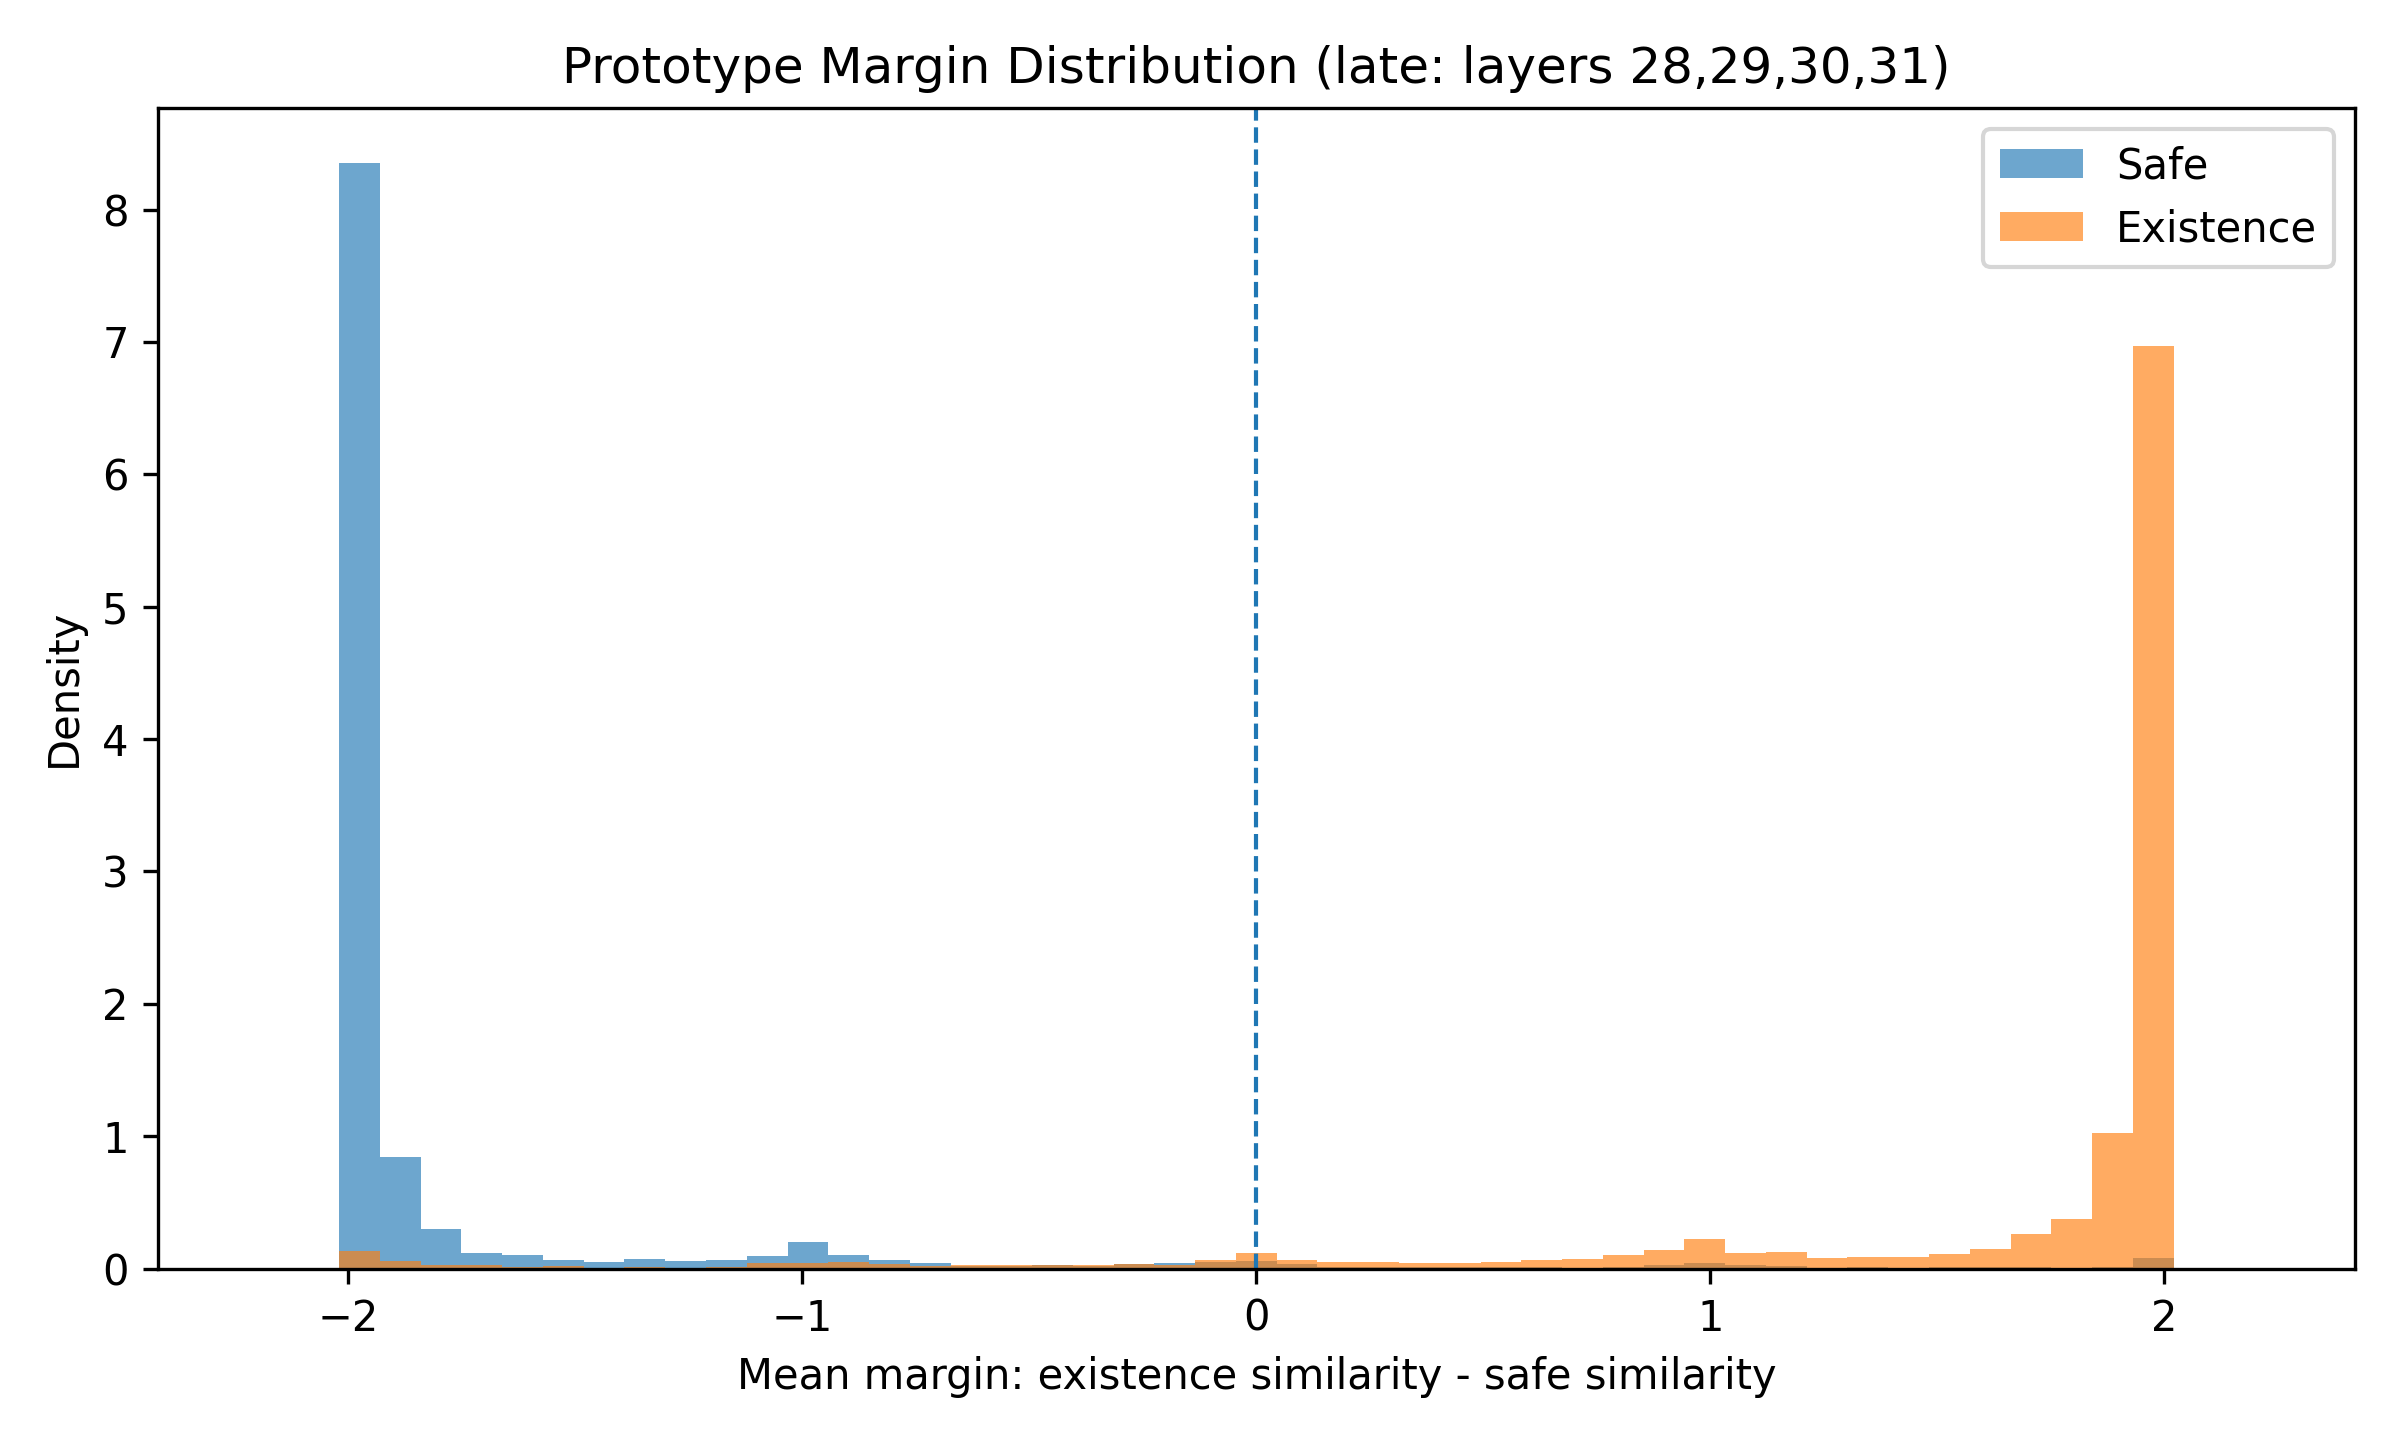
\includegraphics[width=0.32\linewidth]{figures/distribution_late.png}
\caption{Prototype activation distributions across transformer layers.}
\label{fig:distribution}
\end{figure}

Figure~\ref{fig:distribution} shows substantial overlap between Safe and Existence concepts in early layers. However, the separation becomes increasingly clear in middle and deeper layers.

This trend suggests that hallucination-related information becomes progressively more distinguishable as representations move toward higher semantic abstraction levels.



\subsubsection{Limitation}

Although the proposed framework provides meaningful concept-level interpretations of hallucination-related representations, several limitations remain.

\begin{figure}[t]
\centering
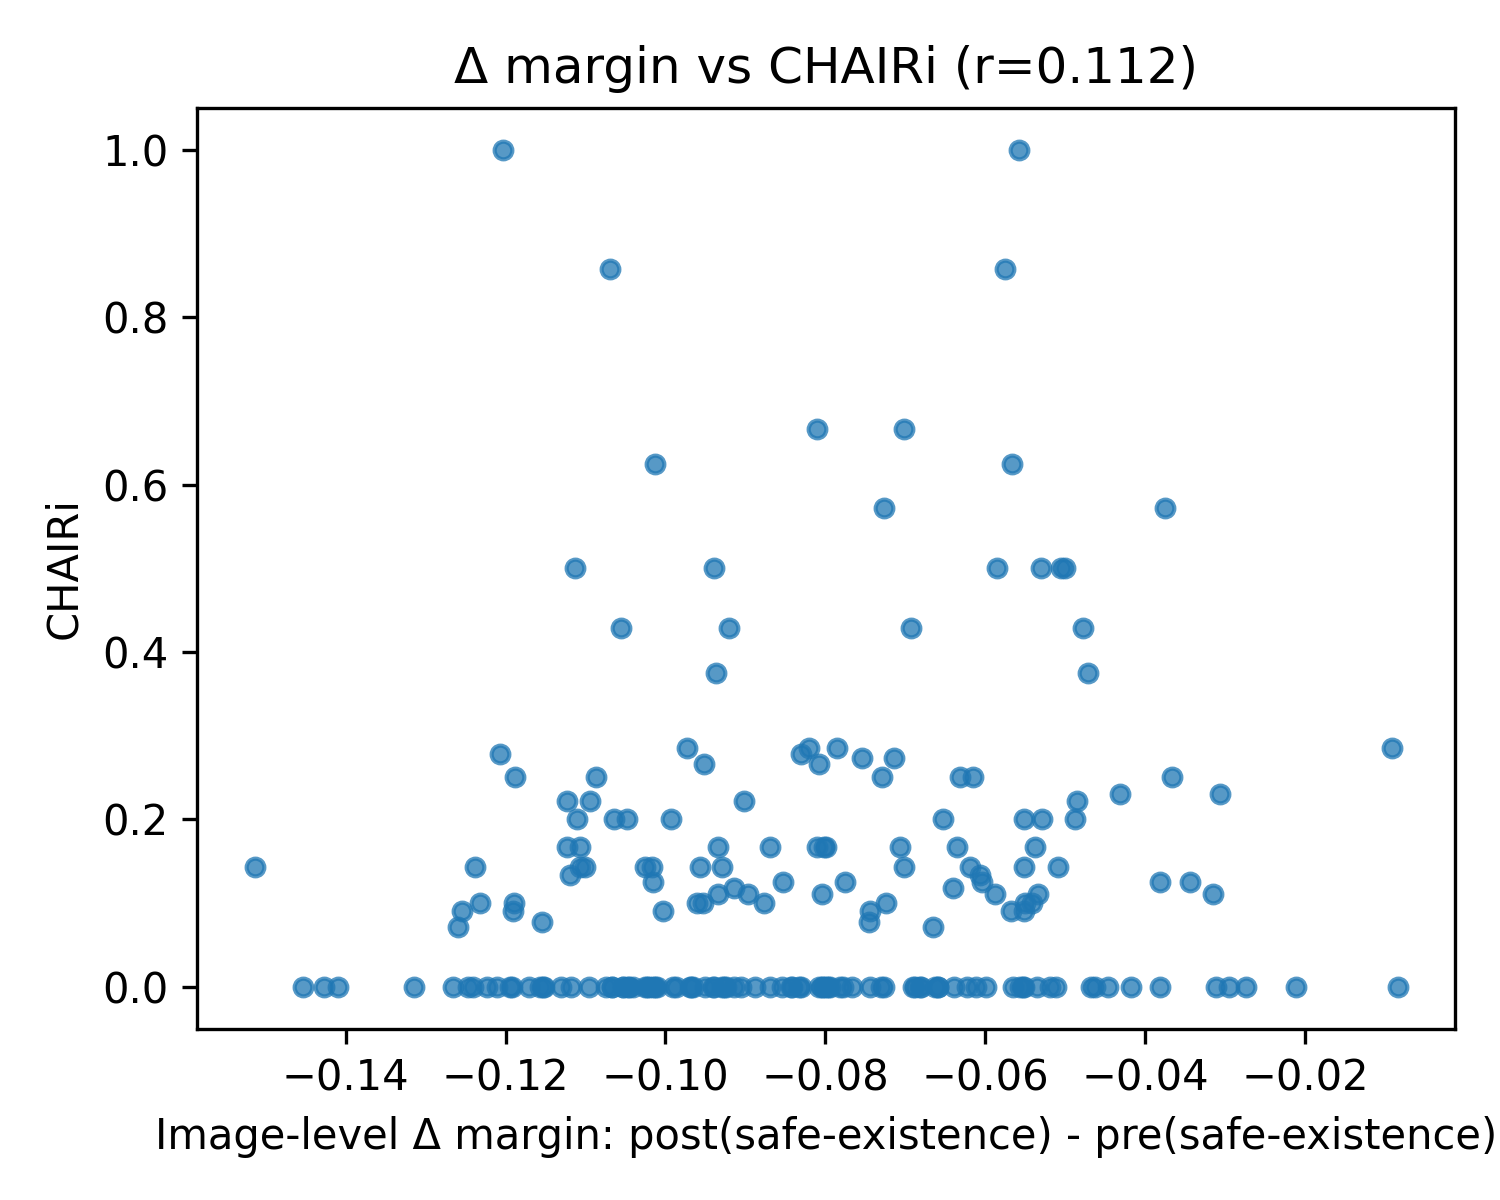
\includegraphics[width=0.48\linewidth]{figures/delta_vs_chairi.png}
\hfill
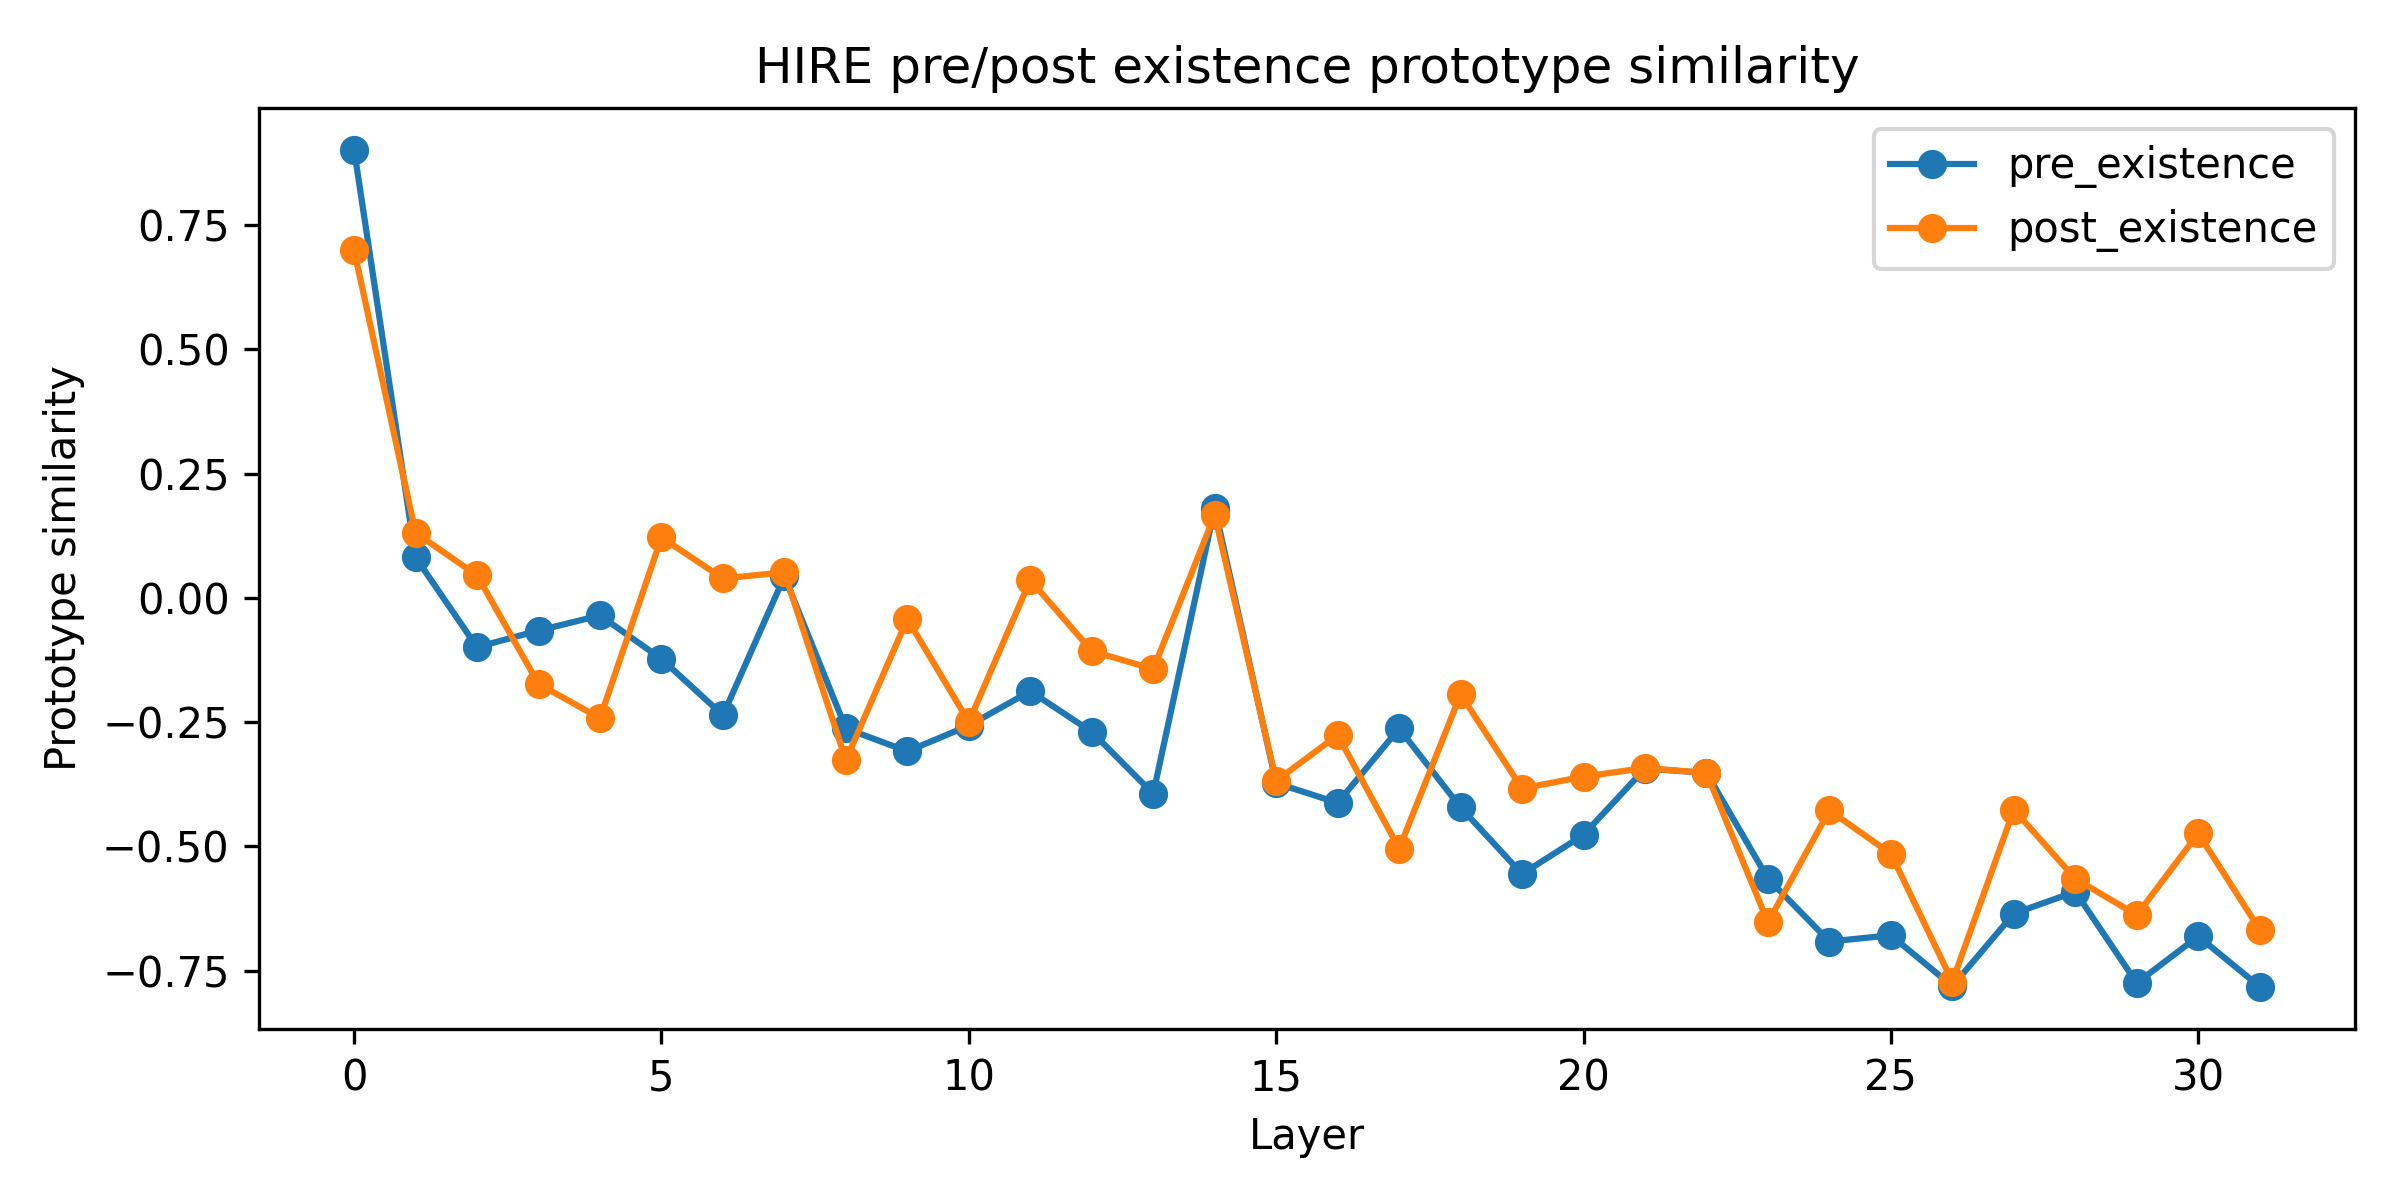
\includegraphics[width=0.48\linewidth]{figures/pre_post_existence_curve.png}
\caption{Limitations of the proposed framework. Left: relationship between concept activation changes and CHAIRi scores. Right: layer-wise Existence concept activations.}
\label{fig:limitation_analysis}
\end{figure}

As shown in Figure~\ref{fig:limitation_analysis}, concept activations exhibit only moderate correlations with hallucination metrics. Furthermore, although Existence activations become increasingly pronounced in deeper layers, the learned concepts are not directly aligned with HIRE's editing objective.

We believe this limitation arises because our framework focuses exclusively on Existence hallucinations, whereas HIRE addresses multiple hallucination categories simultaneously. Consequently, concept activations capture hallucination-related characteristics but remain weakly connected to actual hallucination mitigation performance.

The proposed framework also introduces additional computational overhead due to layer-wise representation extraction and prototype similarity computation.

\begin{table}[t]
\centering
\caption{Inference overhead introduced by the layer-wise CBM module.}
\begin{tabular}{lccc}
\hline
Model & Runtime (s) & With CBM (s) & Overhead \\
\hline
LLaVA & 60 & 352 & 5.87$\times$ \\
HIRE & 139 & 1212 & 8.72$\times$ \\
\hline
\end{tabular}
\label{tab:runtime_results}
\end{table}

As shown in Table~\ref{tab:runtime_results}, the additional analysis module increases inference time by approximately $5.9\times$ to $8.7\times$.

Future work will focus on extending the concept space beyond Existence hallucinations and integrating concept information directly into representation editing frameworks.








\section{Conclusion}

conocnconcocnocnocno

{\small
\bibliographystyle{ieeenat_fullname}
\bibliography{refs}
} 


% WARNING: do not forget to delete the supplementary pages from your submission 
% \input{sec/X_suppl}

\end{document}
